\documentclass{article}
\usepackage{graphicx} % Required for inserting images
\graphicspath{ {./images/} }

\title{Disco Project(CS F222)}
\author{Madhul Aggarwal(2022A7PS1236G)\\ Swetank Rao(2022A7PS0434G) \\ Arul Bhardwaj(2022A7PS1111G)}
\date{30 November 2023}

\begin{document}

\maketitle

\section{Project Report}
\subsection{
Problem Statement
}
We are provided with the problem statement, in which we have to design University Course Assignment System. There are "n" faculty members categorised into three distinct groups: "x1," "x2," and "x3." Faculty in each category are assigned different course loads, with "x1" handling 0.5 courses per semester, "x2" taking 1 course per semester, and "x3" handling 1.5 courses per semester.
In this system, faculty members have the flexibility to take multiple courses in a given semester, and conversely, a single course can be assigned to multiple faculty members. When a course is shared between two professors, each professor's load is considered to be 0.5 courses. Moreover, each faculty member maintains a preference list of courses, ordered by their personal preferences, with the most preferred courses appearing at the top. Importantly, there is no prioritisation among faculty members within the same category. 
\subsection{Objective}
To print five possible optimal cases of allotting faculties.
\subsection{
Required Conditions in Constraints
}

1. The allocation of faculty is randomized and not according to the order of        faculty in the input file.\\
2. The minimum number of courses should be 12.\\
3. All the CDC's should be compulsorily allotted.\\
4. None of the course should be partially filled.\\
5. Electives can be left empty.\\
6. Faculty should be allotted according to their preference list.\\
7. All professors should be fully allotted, in presence of desired number of courses.

\subsection{
Logic implemented 
}
First we will take the number of professors in the university from the user and we will store them in the array data structure. Now we will take the respective faculty types and the respective preferences from the user as input. We will then randomize the array of professors so that they can be allotted randomly. All the data taken as input will be stored in a structure(called faculty in our code). We will then create a function(s) which will create a copy of our vectors and arrays which is storing our inputs so that the original data does not get tampered after certain operations. Allotments are stored in 2D vectors as number of courses is dependent on faculty type. Now we will allot courses to the faculty in the following manner:\\ \\
1. For getting an optimal solution, we will be allotting only 0.5 of a course to the faculty so as to satisfy the preference of the most number of faculties.\\
2. This would require at max 3 iterations as maximum faculty load is 1.5 and we are allotting 0.5 of a course per iteration.\\
3. We iterate through the randomized faculty list so that no faculty gets prioritised first.\\
4. After one complete iteration of the loop, the loop runs two more times for complete allocation.\\
5. All of the data goes through a checking process where if and only if all the constraints are satisfied, then only the program prints the output in the text file.\\
6. Now we will check the remaining course load of each course, if any of the courses is half allotted, the program will not give any output for that case.\\
7. We will then go forward to check to see if courses from CDC's are filled or not. If the latter, then the program wont print any output in this case.\\
8. If all the constraints are satisfied, then the program prints the output in a text file and increases the number of cases by 1.\\
9. It will print outputs until the case number reaches 5.\\



\section{Documentation}
\subsection{Test Case: 1}
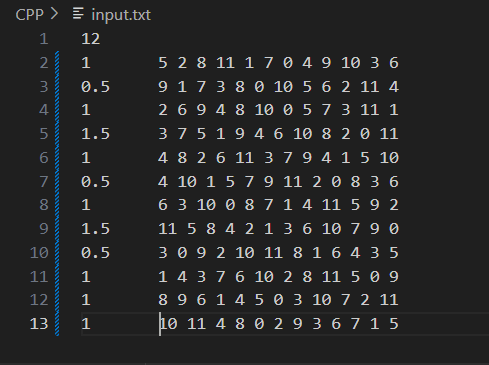
\includegraphics{images/testcase1.png}\\
\subsubsection{There are so many cases possible for the given testcase. One of the "favourable case" is as follows:}
Faculty 1: \\
Iteration 1: 5 -1 -1 -1 -1 -1 -1 -1 -1 -1 -1 -1 \\
Iteration 2: -1 -1 -1 -1 -1 7 -1 -1 -1 -1 -1 -1 \\
Iteration 3: -1\\
Faculty 2: \\
Iteration 1: 9 -1 -1 -1 -1 -1 -1 -1 -1 -1 -1 -1\\ 
Iteration 2: -1\\
Iteration 3: -1\\
Faculty 3: \\
Iteration 1: 2 -1 -1 -1 -1 -1 -1 -1 -1 -1 -1 -1\\ 
Iteration 2: 2 -1 -1 -1 -1 -1 -1 -1 -1 -1 -1 -1 \\
Iteration 3: -1\\
Faculty 4: \\
Iteration 1: 3 -1 -1 -1 -1 -1 -1 -1 -1 -1 -1 -1\\ 
Iteration 2: -1 7 -1 -1 -1 -1 -1 -1 -1 -1 -1 -1 \\
Iteration 3: -1 -1 -1 -1 9 -1 -1 -1 -1 -1 -1 -1 \\
Faculty 5: \\
Iteration 1: 4 -1 -1 -1 -1 -1 -1 -1 -1 -1 -1 -1 \\
Iteration 2: -1 -1 -1 -1 11 -1 -1 -1 -1 -1 -1 -1\\ 
Iteration 3: -1\\
Faculty 6: \\
Iteration 1: 4 -1 -1 -1 -1 -1 -1 -1 -1 -1 -1 -1 \\
Iteration 2: -1\\
Iteration 3: -1\\
Faculty 7: \\
Iteration 1: 6 -1 -1 -1 -1 -1 -1 -1 -1 -1 -1 -1\\ 
Iteration 2: 6 -1 -1 -1 -1 -1 -1 -1 -1 -1 -1 -1 \\
Iteration 3: -1\\
Faculty 8: \\
Iteration 1: 11 -1 -1 -1 -1 -1 -1 -1 -1 -1 -1 -1\\ 
Iteration 2: -1 5 -1 -1 -1 -1 -1 -1 -1 -1 -1 -1 \\
Iteration 3: -1 -1 -1 -1 -1 -1 -1 -1 -1 -1 -1 0 \\
Faculty 9: \\
Iteration 1: 3 -1 -1 -1 -1 -1 -1 -1 -1 -1 -1 -1\\ 
Iteration 2: -1\\
Iteration 3: -1\\
Faculty 10: \\
Iteration 1: 1 -1 -1 -1 -1 -1 -1 -1 -1 -1 -1 -1 \\
Iteration 2: 1 -1 -1 -1 -1 -1 -1 -1 -1 -1 -1 -1 \\
Iteration 3: -1\\
Faculty 11: \\
Iteration 1: 8 -1 -1 -1 -1 -1 -1 -1 -1 -1 -1 -1 \\
Iteration 2: 8 -1 -1 -1 -1 -1 -1 -1 -1 -1 -1 -1 \\
Iteration 3: -1\\
Faculty 12: \\
Iteration 1: 10 -1 -1 -1 -1 -1 -1 -1 -1 -1 -1 -1 \\
Iteration 2: 10 -1 -1 -1 -1 -1 -1 -1 -1 -1 -1 -1\\ 
Iteration 3: -1\\
\subsubsection{Explanation}
1. As we are given with the testcases from the input, we will try to allot courses to the faculties according to the each preference provided by the input.\\
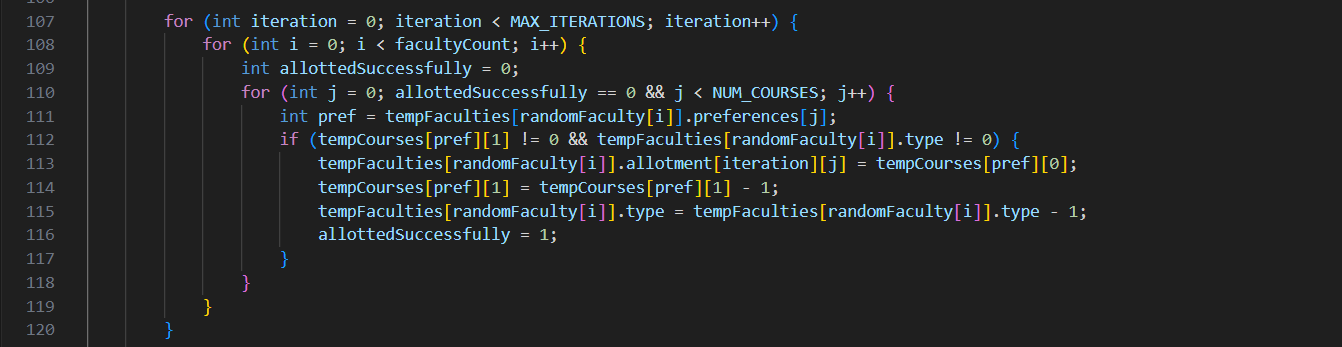
\includegraphics[scale=0.48]{images/allotment.png}\\
2. Course will start allotting half of a course randomly to each faculty according the the preferences provided by them so as to cover priorities of more faculties.\\
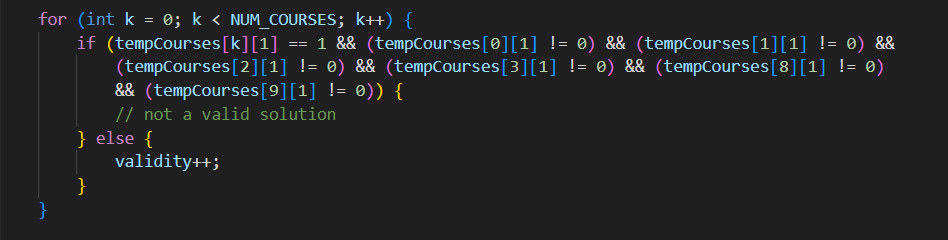
\includegraphics[scale=0.5]{images/constraints.png}\\
3. Now the constraints are going to be checked by our code, if all the conditions satisfies, we will get our output.
\section{Crash Test Report}
\subsection{Case:1}
As the minimum number of faculty capacity can be half of the number of faculty, the maximum number of courses can be 2n, where n is the number of faculty or otherwise a faculty would be alloted no course. \\
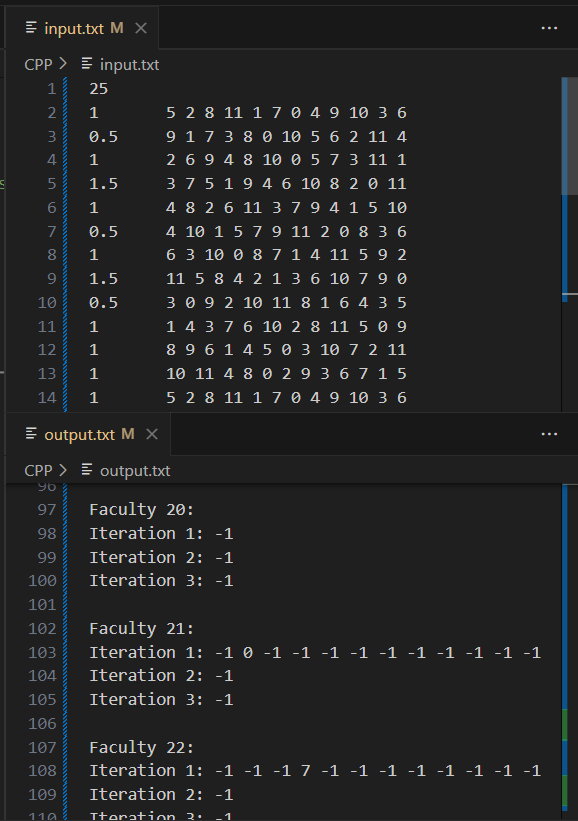
\includegraphics[scale=0.5]{images/crash1.png}\\
\subsection{Case:2}
If we have less number of faculty such that the number of possible cases is less than 5, the program repeated outputs.\\
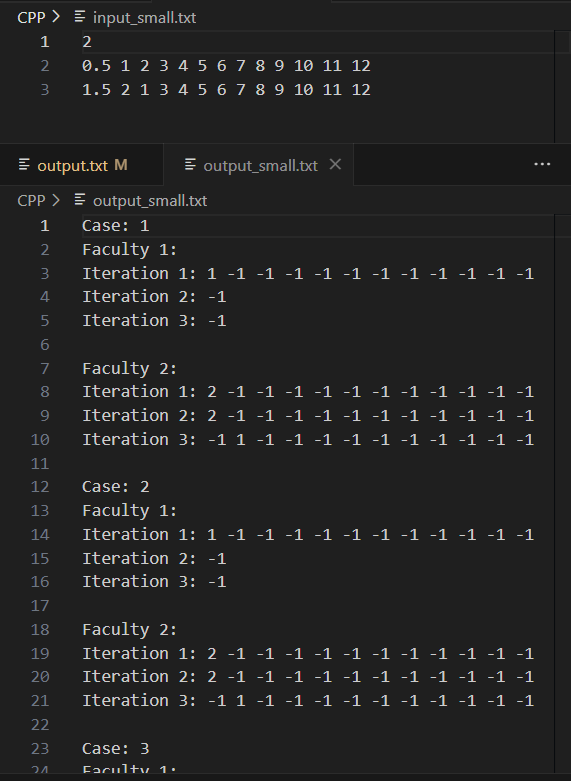
\includegraphics[scale=0.5]{images/crash2.png}\\
\subsection{Case:3}
If we have less number of faculty, then we can not allot all the CDC's which gives no output(goes into an infinite loop).
\subsection{Case:4}
In case of odd multiples of 0.5 (and less number of faculty) some outputs are not feasible, as CDCs constrained is not fulfilled in that case.\\
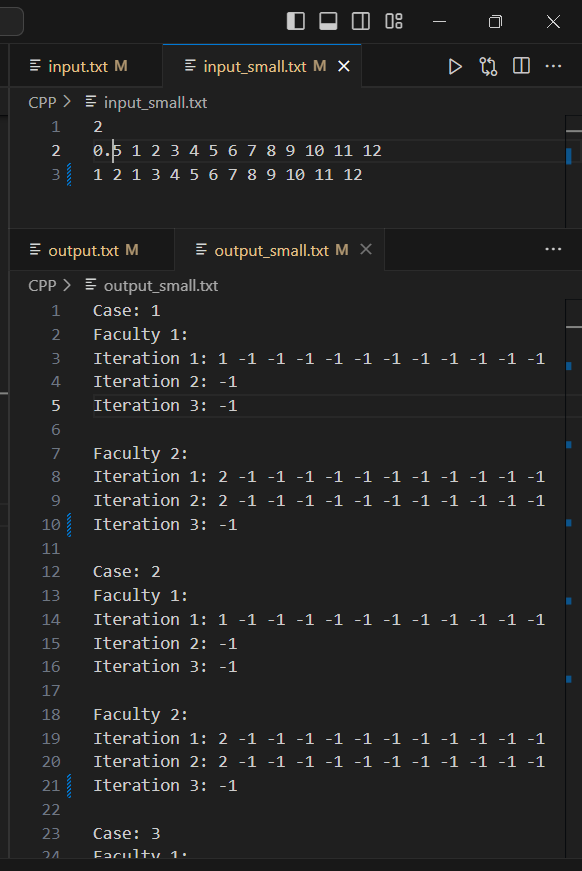
\includegraphics[scale=0.5]{images/crash4.png}\\
\end{document}
